\documentclass{article}%
\usepackage[T1]{fontenc}%
\usepackage[utf8]{inputenc}%
\usepackage{lmodern}%
\usepackage{textcomp}%
\usepackage{lastpage}%
\usepackage{authblk}%
\usepackage{graphicx}%
%
\title{Physical characterisation of Tenacibaculum maritimum for vaccine development}%
\author{Jennifer Kelley}%
\affil{Division of Cardio{-}Vascular Medicine, Department of Internal Medicine, Kurume University School of Medicine, Fukuoka, Japan}%
\date{01{-}01{-}2010}%
%
\begin{document}%
\normalsize%
\maketitle%
\section{Abstract}%
\label{sec:Abstract}%
With its aggressive growth and unfavorable prognosis, lung cancer is quickly becoming a frequent topic of discussion, with many researchers trying to figure out why tumors typically spread even faster than normal tumors. Researchers at Dana{-}Farber Cancer Institute in Boston, MA and the National Cancer Institute at National Institutes of Health in Bethesda, MD. spoke with Miwa Mannu, MD, as part of a series profiling scientists at UCSF and various institutions to discuss their work in lung cancer. Miwa Mannu is the director of the John Greenberg Lung Cancer Research Center at Dana{-}Farber Cancer Institute. She is also a member of the Dana{-}Farber Cancer Institute Medical Ethics and Diversity Council.\newline%
What role do lung cancer cells have in determining what stage of cancer they develop?\newline%
In advance of my work on my personal project, THE HAMM{-}POWER: Aging and the Race to Detect Early{-}Stage Lung Cancer, Lung Cancer, I wanted to better understand the role of adult cells in creating certain early signs of the disease that may indicate which stage of the disease was in progress.\newline%
Where did your research take you?\newline%
Since I started at Dana{-}Farber in 2005, I have been studying lung cancer. I have collaborated with other scientists in various labs at Dana{-}Farber to systematically collect cases, looking for changes in the DNA profile of skin cancer cells that occurred in the fluid of someone with the disease but have not yet developed into normal cells in a human laboratory. After the discovery of DNA molecules that showed they could replicate in cells that had developed into lung cancer cells, I began examining their production and how they function in real life. After more exploratory work, I went on to analyze the ability of the virus known as mucoprotein acid mimin to modify and change the structure of these cells during the early stages of lung cancer. I then investigated the role of mutations that change the genetic makeup of the cell as part of the process to develop lung cancer. I now look to my work in mesothelioma on how mutations in mucoprotein acid mimin can modify and change the behavior of cancer cells.\newline%
How did the research interest you in lung cancer begin?\newline%
I began my nursing studies at SUNY Albany and was not aware at the time of lung cancer. I was diagnosed with early stage lung cancer in 2008. I was aware that a tumour had been found on the surface of my left lung where it had been growing my the past three years. I was then very lucky that it was found immediately and that one of my many nurses was able to do immediate surgery on my lung. Although I have not had advanced lung cancer, my treatment has been poor. I still do lung cancer therapy and my prognosis is not good, although it has improved from a two{-}year survival rate of less than two{-}thirds to five months. I have been clear of any of the current treatments of lung cancer, but some treatments have a deleterious effect on my immune

%
\subsection{Image Analysis}%
\label{subsec:ImageAnalysis}%


\begin{figure}[h!]%
\centering%
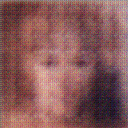
\includegraphics[width=150px]{500_fake_images/samples_5_418.png}%
\caption{A Man With A Beard Wearing A Tie}%
\end{figure}

%
\end{document}